Et skoleskema består af grundlæggende elementer. Som eksempel kan lektioner være et sådanne element, mens tidspunktet for lektionen kan være et andet. Disse grundlæggende elementer er forholdsvist nemme at beskrive, da de er konkrete, og som sagt før, gundlæggende for skoleskemaets opbygning. Der er også mere abstrakte elemtenter i et skoleskema, som hvornår hvilke fag skal lægge tidsmæssigt, både i forhold til hinanden og i forhold til tiden. Det er disse elementer, som kræver mere individuel input, hvis de skal opfylde de krav, som den enkelte bruger stiller.
\\\\
Genetiske algoritmer giver derfor mulighed for let at generere et skoleskema. Som nævnt tidligere bliver mange generationer genereret ud fra parametrer og deres vigtighed overfor 'fitness'-værdien. Dette betyder, at specifikke parametrer kan tages højde for, og det giver større mulighed for fleksibilitet uden at kræve en omvæltning at selve programmet. 

Det er dette koncept, som bærer grundlaget for brugen af genetiske algoritmer til genereringen af skoleskeamer, da programmet helt naturligt speciferer sit resultat til at tilfredsstille de krav, som bliver stillet af brugeren. Dette, samlet med princippet om at kravenes vigtig kan justeres nemt, giver stærkt grundlag for brugen af genetiske algoritmer.



For at lave algoritmen til at planlægge et skema, er der forskellige metoder. Hver metode har fordele og ulemper og er derfor egnet til forskellige problemer.

\subsubsection{Brute Force}

Brute-force algoritmen går i sin simple form ud på, at tjekke alle mulige kombinationer af problemet, og ligesom i den genetiske algoritme, beregne en fitness for hver mulig løsning. Da alle mulige løsninger bliver afprøvet, er det sikkert, at den bedste løsning bliver fundet i forhold til den valgte fitness. 

Hvis der f.eks. skal findes en divisor for et heltal n, ville brute-force metoden gå ud på at gå gennem alle tal mellem 1 og n, og tjekke om tallet kan divideres uden, at producere en rest.

Selvom denne metode er sikker på den optimale løsning, vil et problem med mange parametre kræve længere tid at køre, sammenlignet med andre metoder som genetisk algoritme, da vi i genetisk algoritme hurtigt sorterer mange løsninger fra, uden at gå igennem dem enkeltvis.

Der er visse applikationer hvor brute-force kan være meget brugbart, hvis man F.eks. vil cracke et pass-word. Når man skal cracke et password kan man ikke bruge genetiske algoritmer, for du får ikke et output der fortæller om ens løsning er tæt på at være rigtig. Med brute-force er det sikkert, at man får den rigtige løsning, da brute-force tester alle løsninger.\footfullcite{brute2016}

\subsubsection{Genetiske algoritmer}
Genetiske algoritmer er en metode til at optimere en løsning til et givent problem. Genetiske algoritmer er en række retningslinjer som udefra disse danner flere løsninger til et problem og finde den bedste løsning til problemet.

Genetiske algoritmer er en metode, som er inspireret af Charles Darwins teori om naturlig selektion, som omhandler hvordan de biologiske arter udvikler sig over tid, ved at tilpasse sig miljøet og derved bliver bedre egnet til, at overleve og formere sig i miljøet. Teorien danner grundlag i, at populationen af en given art har forskellige kromosomer og at der over tid vil ske små ændringer i kromosomerne hos individerne. Disse små ændringer i kromosomerne vil over længere tid, føre til større ændringer hos individerne. På daværende tidspunkt var Darwins teori meget kontroversiel, dette er dog ikke tilfældet for softwarebrug af genetiske algoritmer, da en algoritme er noget lettere at forklare, end en biologisk ændring i en art over længere tid.
En genetisk algoritme består af følgende dele.\footfullcite{jebari2013}


1.	Individer som er mulige løsninger til problemet.


2.	Fitness som er en egenskab hos individerne, som bliver udregnet i forhold til, hvor god en løsning individerne er til problemet.


3.	Et individ består af flere kromosomer.


4.	En population som består af en mængde af individer.


5.	Generationer som indikere hvor lang tid algoritmer forløber over.


En population bliver muteret ved følgende operationer:

\paragraph{Selektion}

Operatoren vælger individer til reproduktionen, jo større fitness individerne har, jo større sandsynlighed er der for, at de bliver valgt til reproduktion. Reproduktion kombiner 2 individer og danner ud fra deres kromosomer et nyt individ.\footfullcite{jebari2013}

\paragraph{Crossover}

Operatoren vælger 2 tilfældige kromosomer og blander dem så der bliver dannet 2 nye kromosomer som er en kombination af de 2 kromosomer fx strengene 1110100 1011111 bliver krydset og danner de 2 nye strenge 1010100 1111111.\footfullcite{jebari2013}

\paragraph{Mutation}

Operationen flipper tilfældigt nogle stykker af kromosomet fx strengen 1001000 bliver muteret i dens tredje position til 1011000. Mutation kan ske i alle positioner i strengen med en hvis sandsynlighed. Mutationsprocessen er vigtig for den genetiske algoritme, da man ved at muterer kromosomet udforsker flere muglie løsninger til det givende problem.\footfullcite{jebari2013}
\begin{figure}[!h]
  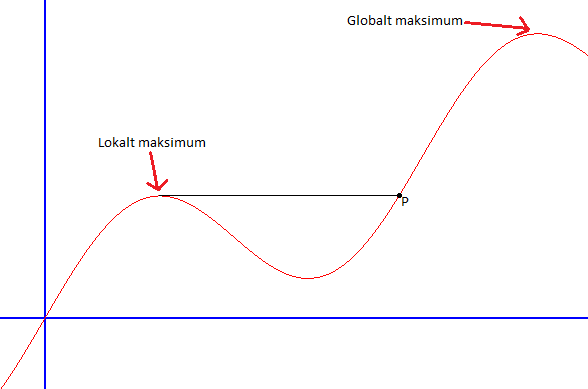
\includegraphics{partials/graphics/lokaltmaksimum.png}
  \caption{Afbildning af variationer af skemaer på x-aksen og fitness værdi på y-aksen}
  \label{fig:Lokalmax}
\end{figure}

På figur~\ref{fig:Lokalmax} ses variationer af skemaer hen ad x-aksen og fitness værdien op af y-aksen. Det første toppunkt markeret med "lokalt maksimum" indikerer et punkt, hvor en variations  har den bedste fitness værdi i forhold til andre tætliggende variationer. Men et globalt maksimum eksisterer også, som indikerer den bedste fitness værdi et skema kan have. Et problem opstår, hvis produktet et fanget i det lokale maksimum. Dette kan forekomme, hvis produktets fitnessværdi ender i det lokale maksimum og der ikke bliver lavet store ændringer nok til at få variationen hen til punktet P. Før punktet P vil variationen ikke være nok til at få en høj fitness værdi. Det er derfor vigtigt, at produktet bliver ændret til en grad, som kan tillade at den kan bryde ud af det lokale maksimum. Det skal bemærkes, at produktet ikke nødvendigvis bliver bedre med en højere variatio, men det gælder om at varierer den nok gange indtil fitness værdien er høj nok. Yderligere skal det bemærkes, at figur~\ref{fig:Lokalmax} skal ses, som en generalisering af princippet og ikke realistisk afbildning. Det er vigtigt, at forstå at variation kan være en stor mængde parametre, som ikke kan afbildes i en 2-dimensionel graf.

\paragraph{Mangfoldighed}

Når den optimale løsning skal findes, er det vigtigt at algoritmen ikke bliver fanget på et lokalt højde-punkt, men at man kan komme over disse til det globale højdepunkt. Eksempelvis, hvis et problem havde 5 parametre, og man udregnede fitness heraf. Heri vil der forekomme selektion, crossover og mutation. Dette betyder at endnu en fitness kan udregnes for den givne population. Men hvad nu, hvis algoritmen hænger fast. 

Hvis parametrene kun ændres en lille smule for hver generation, gør at programmet nu hænger fast, da tallene omkring disse parametre ikke gør at der kommer en højere fitness. Ud fra parametrene muligheden er det mligt at udregne den højeste fitness alt afhængigt af, hvor meget parametrene skal justeres. Minimale ændringer vil ikke nødvendigvis resultere i den højeste fitness, hvorimod store ændringer i parametrene vil muligvis udregne det højeste fitness. Programmet skal i starten gerne finde løsninger, som lægger spredt ud over hele problemet, og så derefter fjerne denne mangfoldighed igen for at ’zoome’ ind på den endelige optimale løsning. 
Det er gavnligt at have er et individ med, ikke bare stor fitness, men et som heller ikke ligner de andre. På figur XX%mangler figur xx
 ses, at der forsøges at finde det individ, der ligger på linjerne.

Både ved brug af brute force og generisk algoritme er målet at finde den optimale løsning. Denne beregnes ud fra et fitness niveau, hvor der på hver løsning laves en udregning ud fra valgte parametre. Denne returnerer et fitnessniveau. Herefter gemmes løsningen med det bedste fitnessniveau. Det bedste fitnessniveau kan være defineret ved den højest mulige eller lavest mulige værdi.\footfullcite{winston2014}

Løsning til problemet.

1.	Der bliver tilfældet generet en population af n-individer med l-kromosomer.


2.	De genetiske algoritme operatorer udsætter populationen for mutation og derved vil der fore-komme ændringer hos kromosomerne i individerne eller danne nye individer.


3.	Der bliver beregnet fitness for hvert n-individ i populationen. Fitness bestemmer sandsynligheden for individet overlever i populationen.


4.	Processen gentages fra trin 2 i x antal givende generationer eller indtil et givet kriterium er opfyldt.


Algoritmen er færdig når x antal generationer er kørt igennem eller et givet kriterium er opfyldt og der vil være en population med potentielle løsninger til problemet, hvor der herudfra vil blive valgt en løsning til problemet som typisk er løsningen med højst fitness. Genetiske algoritmer kan bruges til at optimere problemet med skemalægning, udefra en række retningslinjer som bliver bestemt. Det vil udmunde i en optimal løsning til skemalægningsproblemet, hvis der bliver givet de korrekte retningslinjer.\footfullcite{jebari2013}

\subsubsection{Searchspace}

”Seach space” referer til en gruppe af kandidat løsning til et problem, hvor der er en ”distance” i mellem kandidaterne. For eksempel lad os tage vigtigt problem indenfor bioengeering, hvordan man designer et protein. Antaget at man vil søge efter et protein som er en sekvens af aminosyre som kan blive brugt til at bekæmpe en virus. ”Seach space” vil være en kollektion af alle mulige proteiner. Dette vil give os uendelige mange muligheder derfor begrænser vi længden af proteinet til længden 50 som stadig vil være et stort ”seach space” siden der er 20 mulige aminosyre i hver position i proteinet. Hvis vi repræsenter aminosyrerne i form af alfabetet vil et muligt protein se ledes ud. 
ASDKEGHB…. Vi definer distance mellem proteinerne som forskellen i alfabetet på den tilsvarende position i et andet protein fx ASDKEGHB og BSDKEGHB er distance 1 og distance mellem ASDKEGHB og GCCHAKAA er 8.\footfullcite{jebari2013}
